\documentclass[12pt,a4paper]{article}
\usepackage[utf8]{inputenc}
\usepackage[brazil]{babel}
\usepackage{graphicx}
\usepackage{amssymb, amsfonts, amsmath}
\usepackage{float}
\usepackage{enumerate}
\usepackage[top=1.5cm, bottom=1.5cm, left=1.25cm, right=1.25cm]{geometry}

\newcommand{\sen}{\,\textrm{sen}\,}
\newcommand{\arcsen}{\,\textrm{arcsen}\,}
\newcommand{\tg}{\,\textrm{tg}\,}
\newcommand{\arctg}{\,\textrm{arctg}\,}

\begin{document}
\pagestyle{empty}

\begin{center}
  \begin{tabular}{ccc}
    \begin{tabular}{c}
      
\includegraphics[scale=0.25]{../../biblioteca/imagem/brasao-de-armas-brasil} \\
    \end{tabular} & 
    \begin{tabular}{c}
      Ministério da Educação \\
      Universidade Federal dos Vales do Jequitinhonha e Mucuri \\
      Faculdade de Ciências Sociais, Aplicadas e Exatas - FACSAE \\
      Departamento de Ciências Exatas - DCEX \\
      Disciplina: Cálculo Diferencial e Integral I \quad Semestre: 2021/2\\
      Prof. Me. Luiz C. M. de Aquino\\
    \end{tabular} &
    \begin{tabular}{c}
      
\includegraphics[scale=0.25]{../../biblioteca/imagem/logo-ufvjm} \\
    \end{tabular}
  \end{tabular}
\end{center}

\begin{center}
  \textbf{Lista III}
\end{center}

\begin{enumerate}
 \item Considere a função dada por $f(x) = 3x^3 - 4x$.
 
 \begin{enumerate}
   \item Calcule $f'$ e determine os intervalos de crescimento/decrescimento do gráfico de $f$.
   \item Calcule $f''$ e determine a concavidade do gráfico de $f$.
   \item Use os itens anteriores para fazer um esboço do gráfico de $f$.
 \end{enumerate}
 

 \item Use a primeira derivada para determinar quais funções abaixo são sempre crescentes.
 
 \begin{enumerate}
   \item $f(x) = x^5 + 3x$.
   \item $f(t) = t^7 - t$.
   \item $f(s) = \cos^2 s$.
   \item $f(u) = \sqrt{u} - \dfrac{1}{u}$.
 \end{enumerate}

 \item Use a segunda derivada para determinar quais funções abaixo possuem a concavidade do gráfico
 sempre para baixo.
 
 \begin{enumerate}
   \item $f(x) = x\ln x$.
   \item $f(r) = -r^8 + r$.
   \item $f(t) = -t^2 + \sqrt{t}$.
   \item $f(u) = \dfrac{e^u + e^{-u}}{2}$.
 \end{enumerate}
   
 \item Determine a constante c tal que o gráfico da função dada por $f(x) = \left(1 -\dfrac{2c}{3}\right)x^3 + (3 - 2c)x$ seja sempre decrescente.
 
\end{enumerate}

\newpage
\begin{center}
  \textbf{Gabarito}
\end{center}

\textbf{[1]} 
(a) Crescente: $\left(-\infty,\, -\dfrac{2}{3}\right)$ e $\left(\dfrac{2}{3},\,+\infty\right)$; 
Decrescente: $\left(-\dfrac{2}{3},\, \dfrac{2}{3}\right)$. 
(b) Concavidade para baixo: $\left(-\infty,\, 0\right)$; Concavidade para cima: $\left(0,\, +\infty\right)$. 

(c) 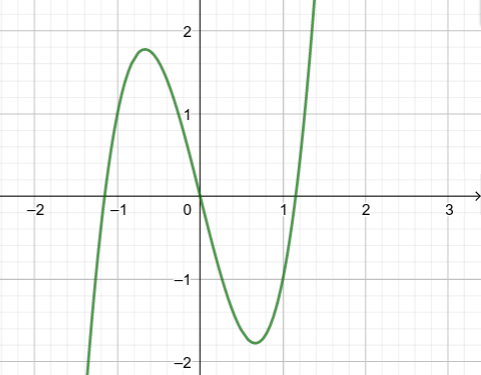
\includegraphics[scale=1]{imagem/grafico-lista-iii-2021.2.png} 

\textbf{[2]} $f(x) = x^5 + 3x$. $f(u) = \sqrt{u} - \dfrac{1}{u}$. 

\textbf{[3]} $f(r) = -r^8 + r$. $f(t) = -t^2 + \sqrt{t}$. 

\textbf{[4]} $c\in \mathbb{R}$, $c > \dfrac{3}{2}$.

\end{document}